\section{Client Design}

\subsection{Design of Client Structure}

\subsection{Outline}

This section will outline our initial design of the system. We aimed for a high degree of modularity to separate concerns among team members and improve the ease of maintaining code. The process of identifying the concerns of the client and representing these in a component based design will be discussed in the `Approach' section. The remainder of the section will discuss our design of individual components, and how we identified their roles within the larger system. Particular focus will be made on how we made sure sections of the client were removed as far as possible from other sections, and challenges in ensuring this requirement. 

\subsection{Approach}

In designing the client, we had the high level aim of creating a modular system to allow team members to take responsibility for certain aspects of the system. From an early stage in the design process, we were aware that the client had a large set of responsibilities. We determined these responsibilities to be: to maintain a connection with the server, implement the GIM protocol, provide a user interface to the system and keep a record of up to date information about the user's friends. Our first task was to design a set of interacting sub-components to handle these responsibilities.

It was agreed that the MVC (Model-View-Controller) architectural pattern, widely used for applications involving a graphical user interface, was a useful model to base our discussions around. This model abstracts the UI (view) from the back end of the system. When a user performs an action, the controller updates the model if any data associated with the system is changed, and updates the viewer to reflect these changes in the system state. This seemed appropriate to our needs of keeping and displaying an up-to-date record of the user's friend list and creating an interface, and would allow us to split responsibilities between the back and front end of the GUI.

However, we faced challenges in creating an additional networking component to implement the GIM protocol into this framework. We had the choice to conceptualise it as either an additional interface, which `viewed' changes to the model, or indirectly (by way of the network) as a part of the controller component. [discussion about possible merits of both goes here] We decided it would be useful to treat the networking code as part of the controller, as it would be modifying the model based on the server's response to its calls, and modifying the GUI to reflect these changes.
	
This high level approach allowed us to draw boundaries between components and assign the more detailed design of individual components to team members. We decided a logical split would be to assign two members to the networking aspects of the system (client and server), and two members to the GUI components of the system (the GUI and its model). However, further collaboration was required as it became more evident what was required for each component, as will be discussed.

[Diagram goes here, reflecting the above discussion (???) ]

\subsection {Model-Viewer-Controller Structural Concerns}

\subsection {Controller}

The controller was one of the more challenging parts of the design process. The controller would be called by both the networking component and the viewer, implying that its operations must be thread safe. We were constrained by our use of the Java Swing\footnote{See \texttt{http://download.oracle.com/javase/6/docs/technotes/guides/swing/} for more information.} environment, which we had learned from previous experience will freeze if the networking code is run on the GUI thread. A further complexity was handling the boundary between the requirements of the network code and the protocol that was being handled by the networking code. Naturally, the GUI architects should not need to concern themselves with the specifics of the protocol while designing the GUI. 

To deal with the threading complexity, we designed a scheme with an intermediate buffer between the controller component and the networking code. The controller thread waits until there is a command from the network placed into the buffer, and acts accordingly on the model and GUI. Furthermore, when the controller component needs to call the network, it places a command into the buffer to be interpreted by the networking code. We believed this scheme to be appropriate as the controller could either call the network from internal code or events from the GUI (possibly simultaneously).\footnote{See networking design section(***use labels here***) for further discussion on the motivation behind this buffer.}

[confusing] To deal with the design complexity of the boundary, we decided that initially, an interface would be written by the networking architects to describe the requirements of the GIM protocol of the client from the controller. The controller would then implement this interface. This allowed the requirements from the client to be understood, without having to understand the inner workings of the protocol. Furthermore, the structure of the protocol could change, without any change to the interface or consultation with the GUI architects. The networking architect would write a method in the controller class to parse incoming commands to call the methods described by the interface as appropriate. For outgoing commands to the server, an interface outlining possible calls to the server would be written by the architect to be called by the controller. [/confusing (restructure sentences, basically)]

note: not final version
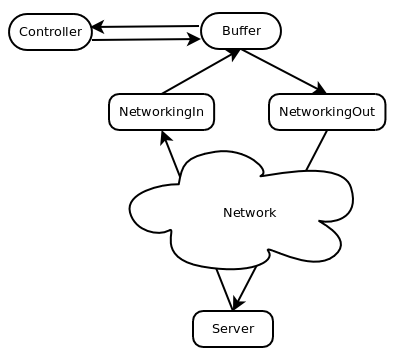
\includegraphics[scale=0.65]{Design/diagrams/buffer.png}

\subsection {Model}

The design of the model involved determining what state information had to be held about the client. This was informed by the previous work of requirements analysis and the conception of features. The model was also informed by the design of the viewer.

Two ``must haves'' of the system were the presence of a contact list and support for user statuses. This implied that there should be data structures for these items. To deal with this requirement, we designed the model to have a data structure to maintain information about users, including their status, nickname and personal messages. 

The view required that the user's own state information (such as status and nickname) were displayed. As these were evident in multiple windows in the view design (such as in chat windows, and on the buddy list), the model was designed to maintain a record of the user's current status. 

\subsection {Viewer}

After some interface design work (which will be discussed in coming sections), it was apparent that the system had to support two different styles of chat windows: a group chat and a chat with a single user. However, there were some observable commonalities between both windows, such as sending messages, displaying incoming messages, and using very similar Java Swing components to handle this functionality. At the same time, there was enough differing behaviour between the two windows to justify having two different classes to handle them, such as the group chat's need to maintain a list of users in the room. With this in mind, we designed our class structure code dealing with the interface to have a super class named ChatWindow, outlining this common functionality, which two sub classes called GroupChatWindow and SingleChatWindow which would extend this super class. [except we chose this later, initially they were the same class, then separate classes, then a super->sub class pattern... another change to discuss, maybe?]%footnote for java swing?

We anticipated this would be advantageous as it would reduce the repetition of code and keep functionality consistent between the two windows. We felt in particular that the panel displaying incoming images would change in formatting messages, as the project would evolve to include some of our possible features, such as the implementation of emoticons and font colours (See section x.y). [this last sentence is confusing... reword?]

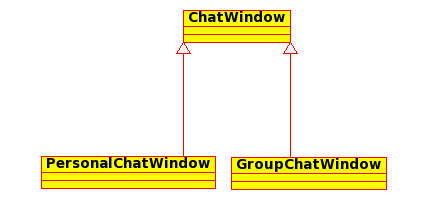
\includegraphics[scale=0.65]{Design/diagrams/chatwin.png}




\subsection{Design of GUI}

As we had decided to incorporate both group and one-to-one chats, this provided a wide scope in terms of interface design. We had the option to base our interface on either IRC or Windows Live Messenger style clients, or to create something entirely of our own. Windows Live was ultimately selected as the basis of the GUI for a number of reasons; primarily we believed that it was better suited to our feature set. An IRC style interface would require a considerable amount of redesigning to accommodate features such as display pictures, contact lists, and offline messaging. While creating our own style of IM interface would be interesting, it would likely lead to an inferior design, and be more time consuming to create. Windows Live style programs typically integrate the vast majority--if not all--of our MoSCoW feature set, and was therefore chosen as our starting point.
 
After we had decided the basic form of the interface, we created use cases for the client interactions. As all users have equal rights within the application we did not deem it necessary to produce diagram representations.

\subsubsection{Example Use Cases}

The following are examples of key use cases:


